\section{Check bitstream functionality}

\label{check}

To check bitstream functionality the serial terminal CuteCom \cite{gh:cutecom} is used but it would be similar with other serial terminals.

\vspace{5mm}

\noindent When the bitstream is loaded to Arty board through command \ref{cod:7} the CuteCom terminal can be opened to check that the Prompt (generated by NEORV32 bootloader) is printed correctly via UART.
That is, the generated bitstream through FLOS tools works successfully. 

\vspace{5mm}

\noindent \textbf{WARNING} If this is the first time you are performing a UART communication in Linux, you should take into account the following: the \say{dialout} user must be added. This is done through the following command: 

\begin{code}
\begin{minted}[frame=lines,framesep=2mm,baselinestretch=1.2,fontsize=\footnotesize,breaklines]{bash}
sudo usermod -aG dialout $USER
\end{minted}
\caption{Command to add dialout user.}
\label{cod:9}
\end{code}

\vspace{5mm}

\noindent Then restart computer or apply command \mintinline[breaklines]{bash}{exec newgrp dialout} and check through \mintinline[breaklines]{bash}{groups} command that the user \say{dialout} is added.

\vspace{5mm}

\noindent After the bitstream is loaded open CuteCom program, set device (/dev/tty/USBx \footnote{Remplace \say{x} with the number that has been associated with your board.}), adjust the settings (Bauderate: 19200, Data bits: 8), open UART communication and if you've followed the example you should see from the terminal something similar to what is shown in figure \ref{fig:cute}.

\begin{figure}[H]
    \centering
    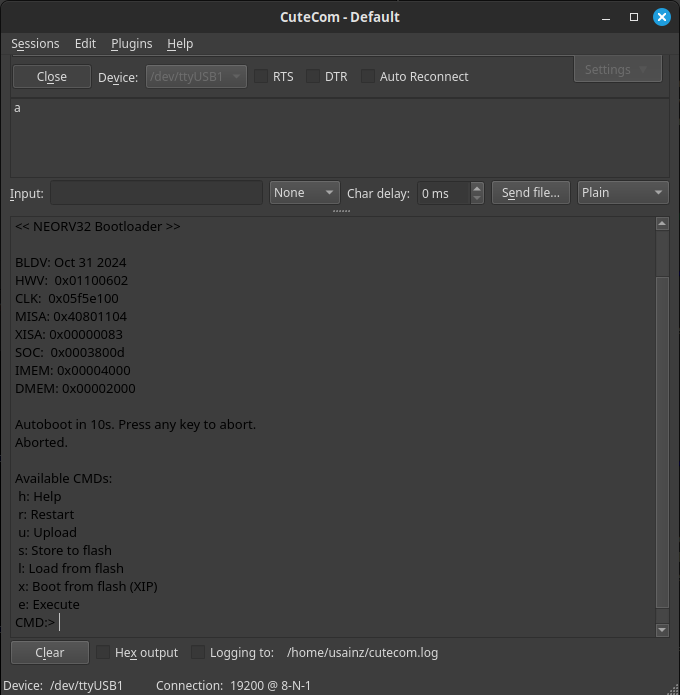
\includegraphics[width=150mm]{figures/res.png}
    \caption{CuteCom result.}
    \label{fig:cute}
\end{figure}
